\documentclass[14pt,a4paper,report]{report}
\usepackage[a4paper, mag=1000, left=2.5cm, right=1cm, top=2cm, bottom=2cm, headsep=0.7cm, footskip=1cm]{geometry}
\usepackage[utf8]{inputenc}
\usepackage[english,russian]{babel}
\usepackage{indentfirst}
\usepackage[dvipsnames]{xcolor}
\usepackage[colorlinks]{hyperref}
\usepackage{listings} 
\usepackage{fancyhdr}
\usepackage{caption}
\usepackage{graphicx}
\hypersetup{
	colorlinks = true,
	linkcolor  = black
}

\usepackage{titlesec}
\titleformat{\chapter}
{\Large\bfseries} % format
{}                % label
{0pt}             % sep
{\huge}           % before-code


\DeclareCaptionFont{white}{\color{white}} 

% Listing description
\usepackage{listings} 
\DeclareCaptionFormat{listing}{\colorbox{gray}{\parbox{\textwidth}{#1#2#3}}}
\captionsetup[lstlisting]{format=listing,labelfont=white,textfont=white}
\lstset{ 
	% Listing settings
	inputencoding = utf8,			
	extendedchars = \true, 
	keepspaces = true, 			  	 % Поддержка кириллицы и пробелов в комментариях
	language = C,            	 	 % Язык программирования (для подсветки)
	basicstyle = \small\sffamily, 	 % Размер и начертание шрифта для подсветки кода
	numbers = left,               	 % Где поставить нумерацию строк (слева\справа)
	numberstyle = \tiny,          	 % Размер шрифта для номеров строк
	stepnumber = 1,               	 % Размер шага между двумя номерами строк
	numbersep = 5pt,              	 % Как далеко отстоят номера строк от подсвечиваемого кода
	backgroundcolor = \color{white}, % Цвет фона подсветки - используем \usepackage{color}
	showspaces = false,           	 % Показывать или нет пробелы специальными отступами
	showstringspaces = false,    	 % Показывать или нет пробелы в строках
	showtabs = false,           	 % Показывать или нет табуляцию в строках
	frame = single,              	 % Рисовать рамку вокруг кода
	tabsize = 2,                  	 % Размер табуляции по умолчанию равен 2 пробелам
	captionpos = t,             	 % Позиция заголовка вверху [t] или внизу [b] 
	breaklines = true,           	 % Автоматически переносить строки (да\нет)
	breakatwhitespace = false,   	 % Переносить строки только если есть пробел
	escapeinside = {\%*}{*)}      	 % Если нужно добавить комментарии в коде
}

\begin{document}

\def\contentsname{Содержание}

% Titlepage
\begin{titlepage}
	\begin{center}
		\textsc{ФЕДЕРАЛЬНОЕ ГОСУДАРСТВЕННОЕ АВТОНОМНОЕ ОБРАЗОВАТЕЛЬНОЕ УЧРЕЖДЕНИЕ ВЫСШЕГО ОБРАЗОВАНИЯ
«САНКТ-ПЕТЕРБУРГСКИЙ ПОЛИТЕХНИЧЕСКИЙ УНИВЕРСИТЕТ ПЕТРА ВЕЛИКОГО»\\[5mm]
			Институт компьютерных наук и технологий\\
			Высшая школа интеллектуальных систем и суперкомпьютерных технологий}
		
		\vfill
		
		\textbf{Дисциплина «Цифровые ресурсы в научных исследованиях»\\[10mm]
		ОТЧЕТ\\[2mm]
		по практической работе №1\\[2mm]
		на тему\\[2mm]
			«Работа с библиотечным сайтом, освоение основных предоставляемых услуг»\\[41mm]
		}
	\end{center}
	
	\hfill
	\begin{minipage}{.4\textwidth}
		Выполнил:\\[2mm] 
        Студент группы 3540901/02001\\
		Дроздов Н.Д.\\[2mm]
        «....» ................... 2020г., ...............\\
        \hspace*{38mm} (Подпись)\\[2mm]
		Проверил:\\[2mm] 
		Бендерская Е.Н.\\[2mm]
		«....» ................... 2020г., ...............\\
        \hspace*{38mm} (Подпись)\\
	\end{minipage}
	\vfill
	\begin{center}
		Санкт-Петербург\\ \the\year\ г.
	\end{center}
\end{titlepage}

% Contents
\tableofcontents
\clearpage

\chapter{Практическая работа №1}

\section{Цель работы}

Получение навыков работы с библиотечным сайтом.

\section{Задачи}

\begin{enumerate}
	
	\item Изучение принципов распределения информационно-библиотечных ресурсов и сервисов, ориентированных на студента, на библиотечном портале.
	
	\item Освоение основных приемов поиска информационных ресурсов в различных источниках, доступных на библиотечном портале.
	
\end{enumerate}

\clearpage

\section{Ход работы}

\subsection{Упражнение 1. Библиотечный портал СПбПУ}

\subsubsection{Найти места расположения ссылок на библиотечный портал на сайте университета.}

Ввели термин «информационно-библиотечный комплекс» в строку поиска на главной странице сайта университета.

\begin{figure}[h!]
\centering

\includegraphics[scale = 0.33]{111.png}
\caption{Поиск по сайту СПбПУ.}
\label{image:1}
\end{figure}

\begin{figure}[h!]
\centering
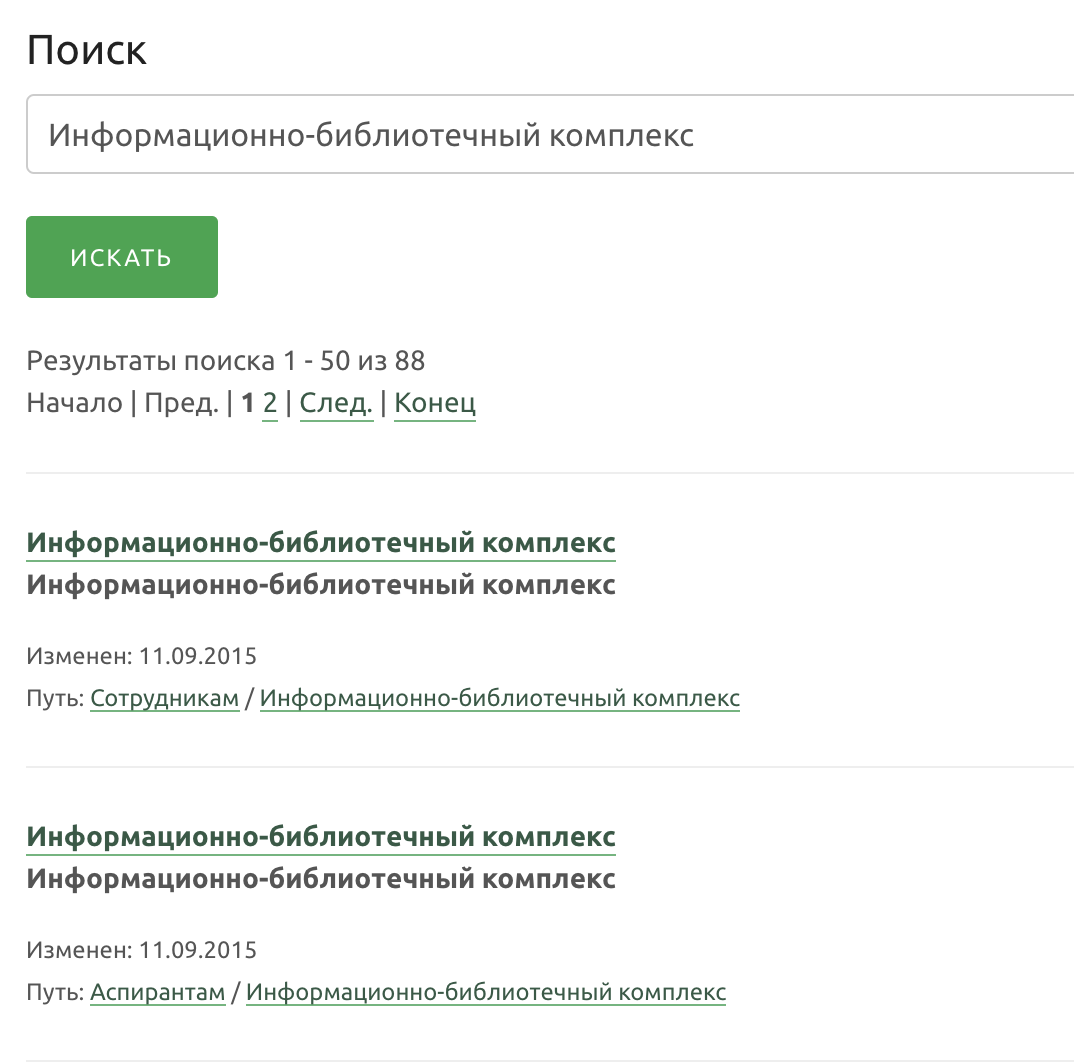
\includegraphics[scale = 0.5]{112.png}
\caption{Результаты поиска библиотечного портала на сайте СПбПУ.}
\label{image:1}
\end{figure}

Определили другие ссылки на библиотечный портал с сайта университета.

\begin{figure}[h!]
\centering

\includegraphics[scale = 0.33]{113.png}
\caption{Поиск по сайту СПбПУ.}
\label{image:1}
\end{figure}

\clearpage

В результате можно найти такую ссылку.

\begin{figure}[h!]
\centering
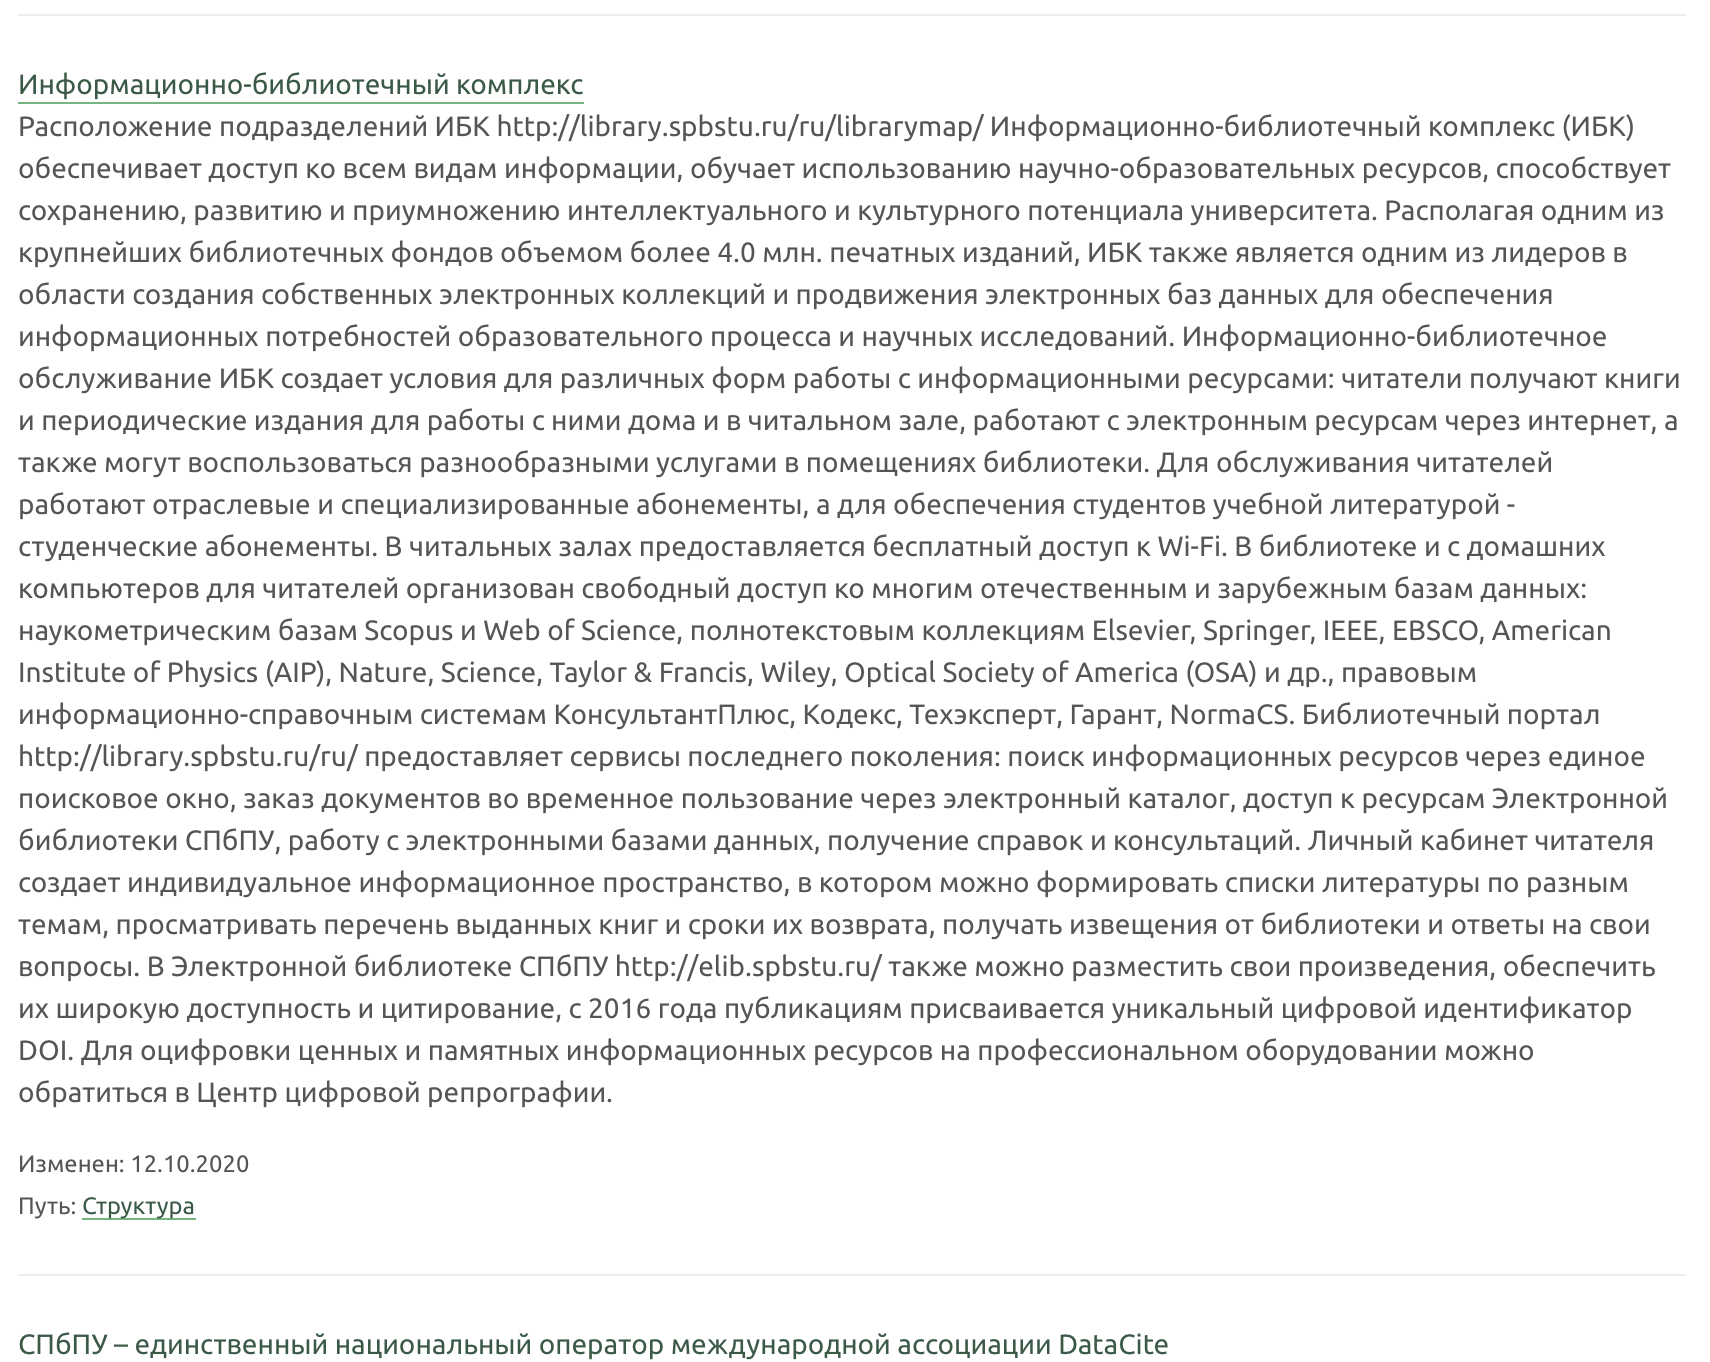
\includegraphics[scale = 0.5]{114.png}
\caption{Результаты поиска библиотечного портала на сайте СПбПУ.}
\label{image:1}
\end{figure}

\clearpage

\subsubsection{Найдите библиотечный портал СПбПУ, пользуясь поисковой машиной Интернет, например, Google.}

Ввели термин «библиотечный портал СПбПУ» в строку поиска Google.

\begin{figure}[h!]
\centering
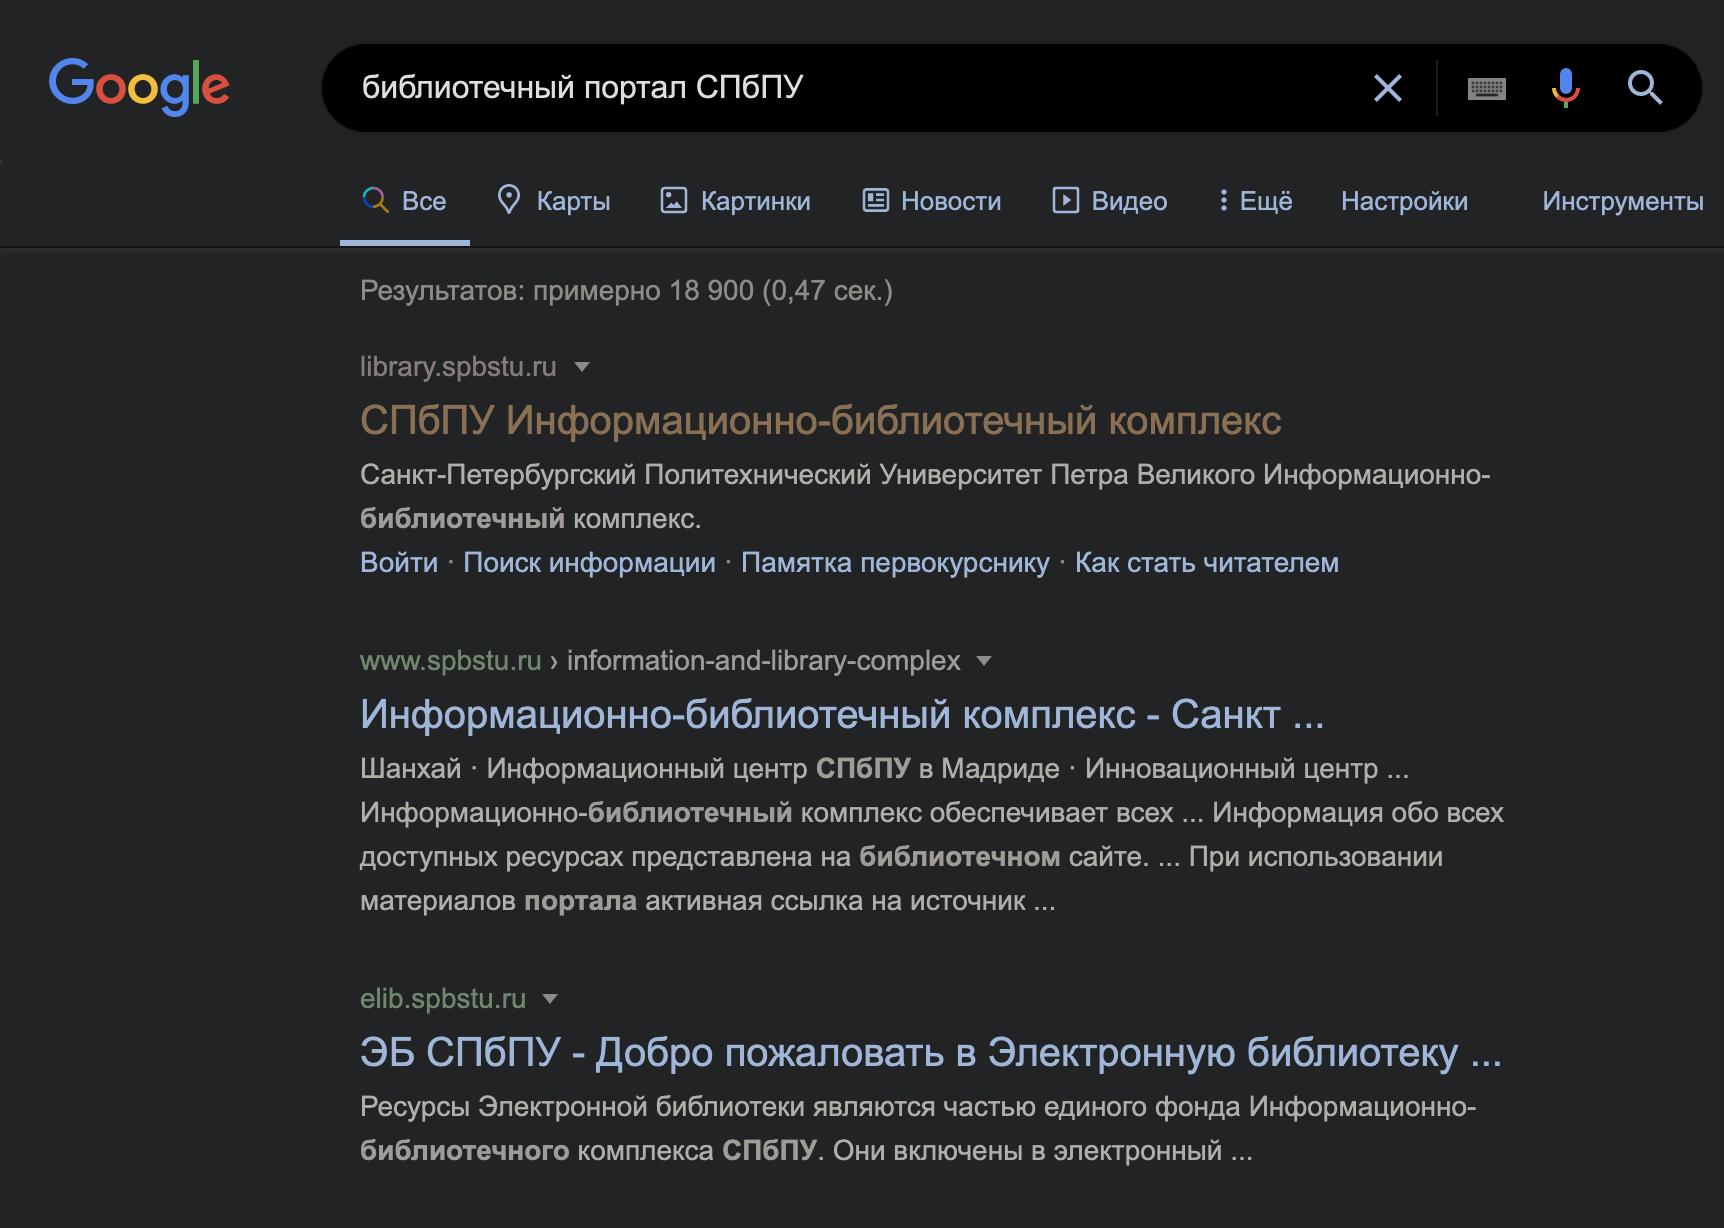
\includegraphics[scale = 0.5]{115.png}
\caption{Результаты поиска библиотечного портала СПбПУ с использованием Google.}
\label{image:1}
\end{figure}

Все результаты, представленные в верхней части списка, ведут или непосредственно к библиотечному порталу, или к страницам, где есть прямая ссылка на него.

\clearpage

Самостоятельно выполнили поиск библиотечного портала с использованием поисковых машин Интернет, пользуясь иными терминами для поиска.

\begin{figure}[h!]
\centering
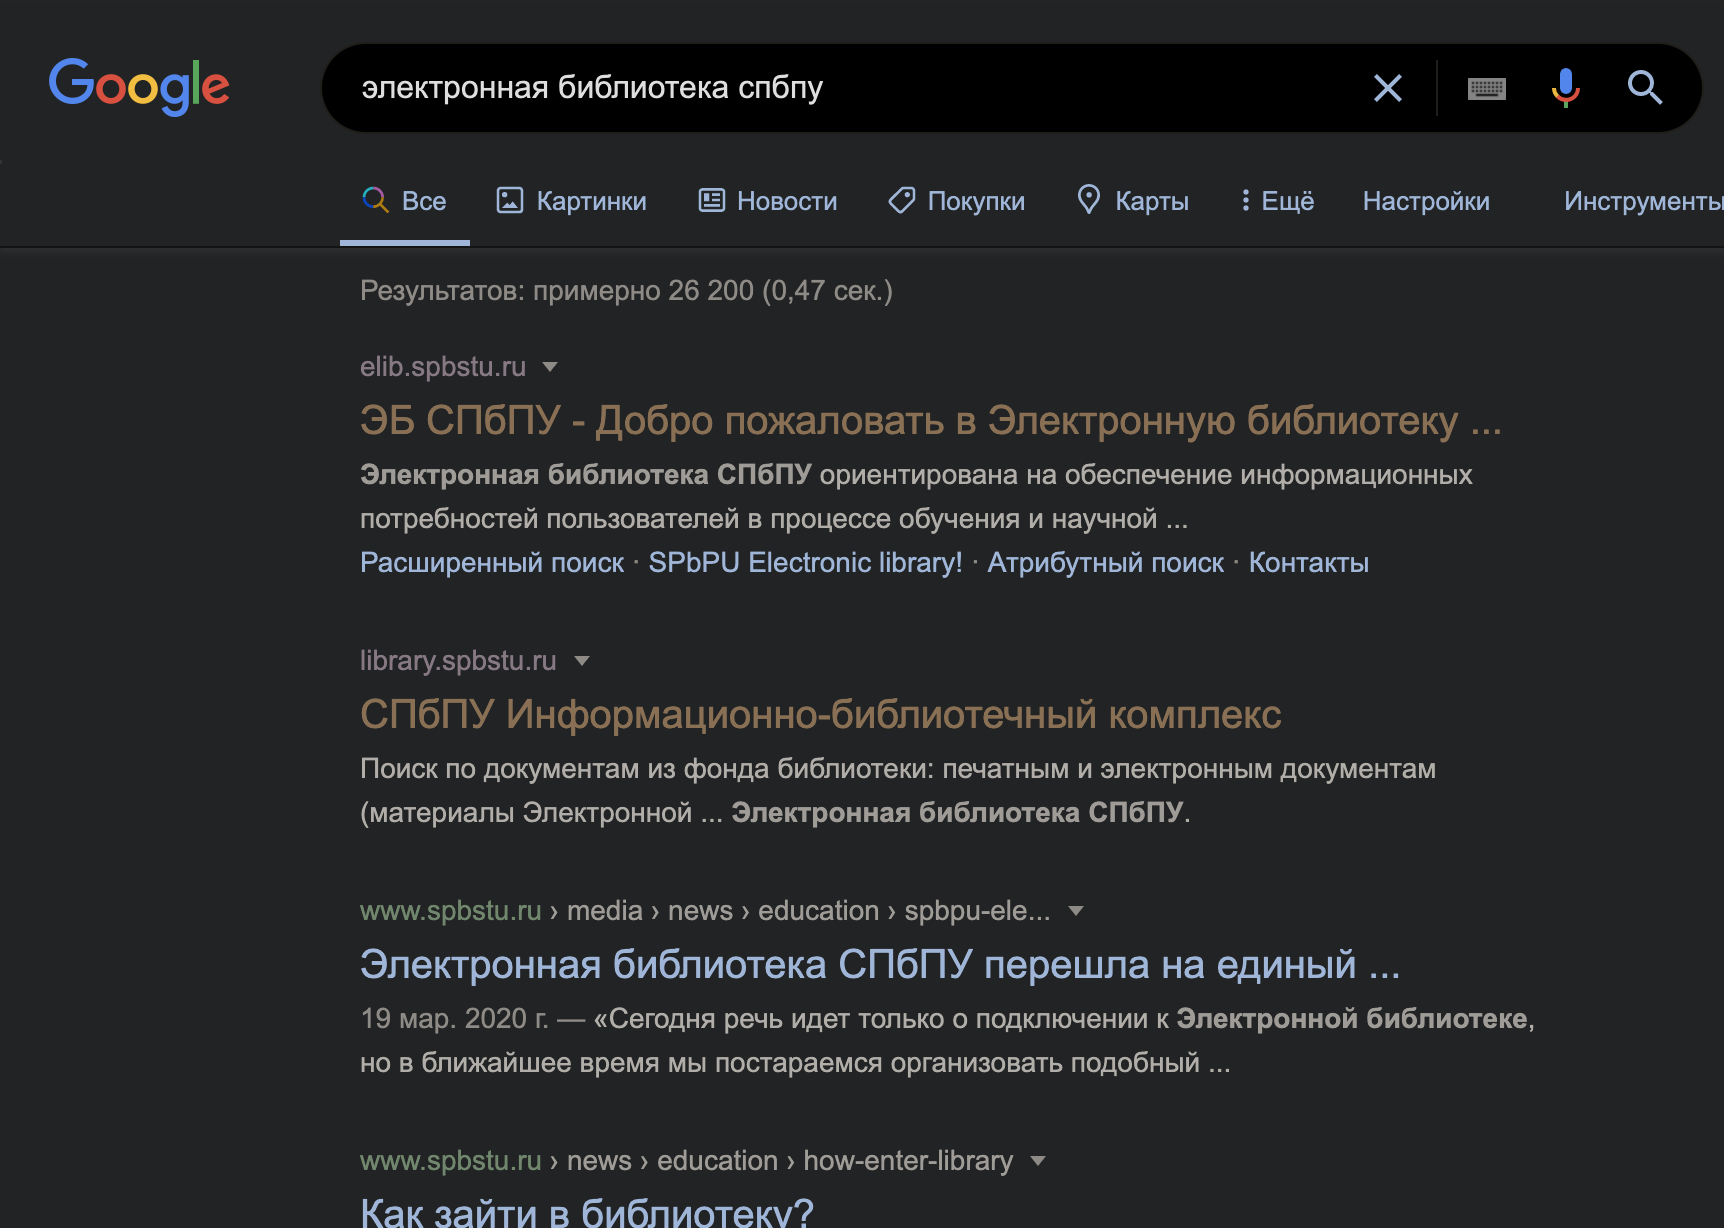
\includegraphics[scale = 0.5]{116.png}
\caption{Результаты поиска библиотечного портала СПбПУ с использованием Google и иным термином для поиска.}
\label{image:1}
\end{figure}

\subsection{Упражнение 2. Поиск информации (описательной) на библиотечном портале}

\subsubsection{Найти расположение отделов библиотеки (абонементов), где можно получить учебники, рекомендованные преподавателем.}

На главной странице изучили раздел объявлений, где в начале учебного года размещается особое расписание обслуживания первокурсников.
Уточнили абонементы, на которых выдаются книги студентам института (школы). Для этого в пунктах меню "Об ИБК" - "Структура" - "Отдел учебной литературы" выбрали подразделение (сектор), направленное на обслуживание обучающихся разных направлений подготовки.

\begin{figure}[h!]
\centering
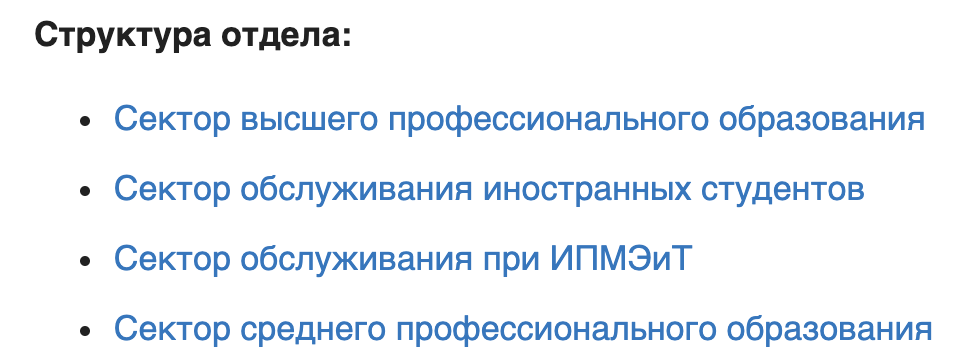
\includegraphics[scale = 0.5]{121.png}
\caption{Структура отдела учебной литературы.}
\label{image:1}
\end{figure}

\clearpage

Для примера, выбрали "Сектор высшего профессионального образования".

\begin{figure}[h!]
\centering
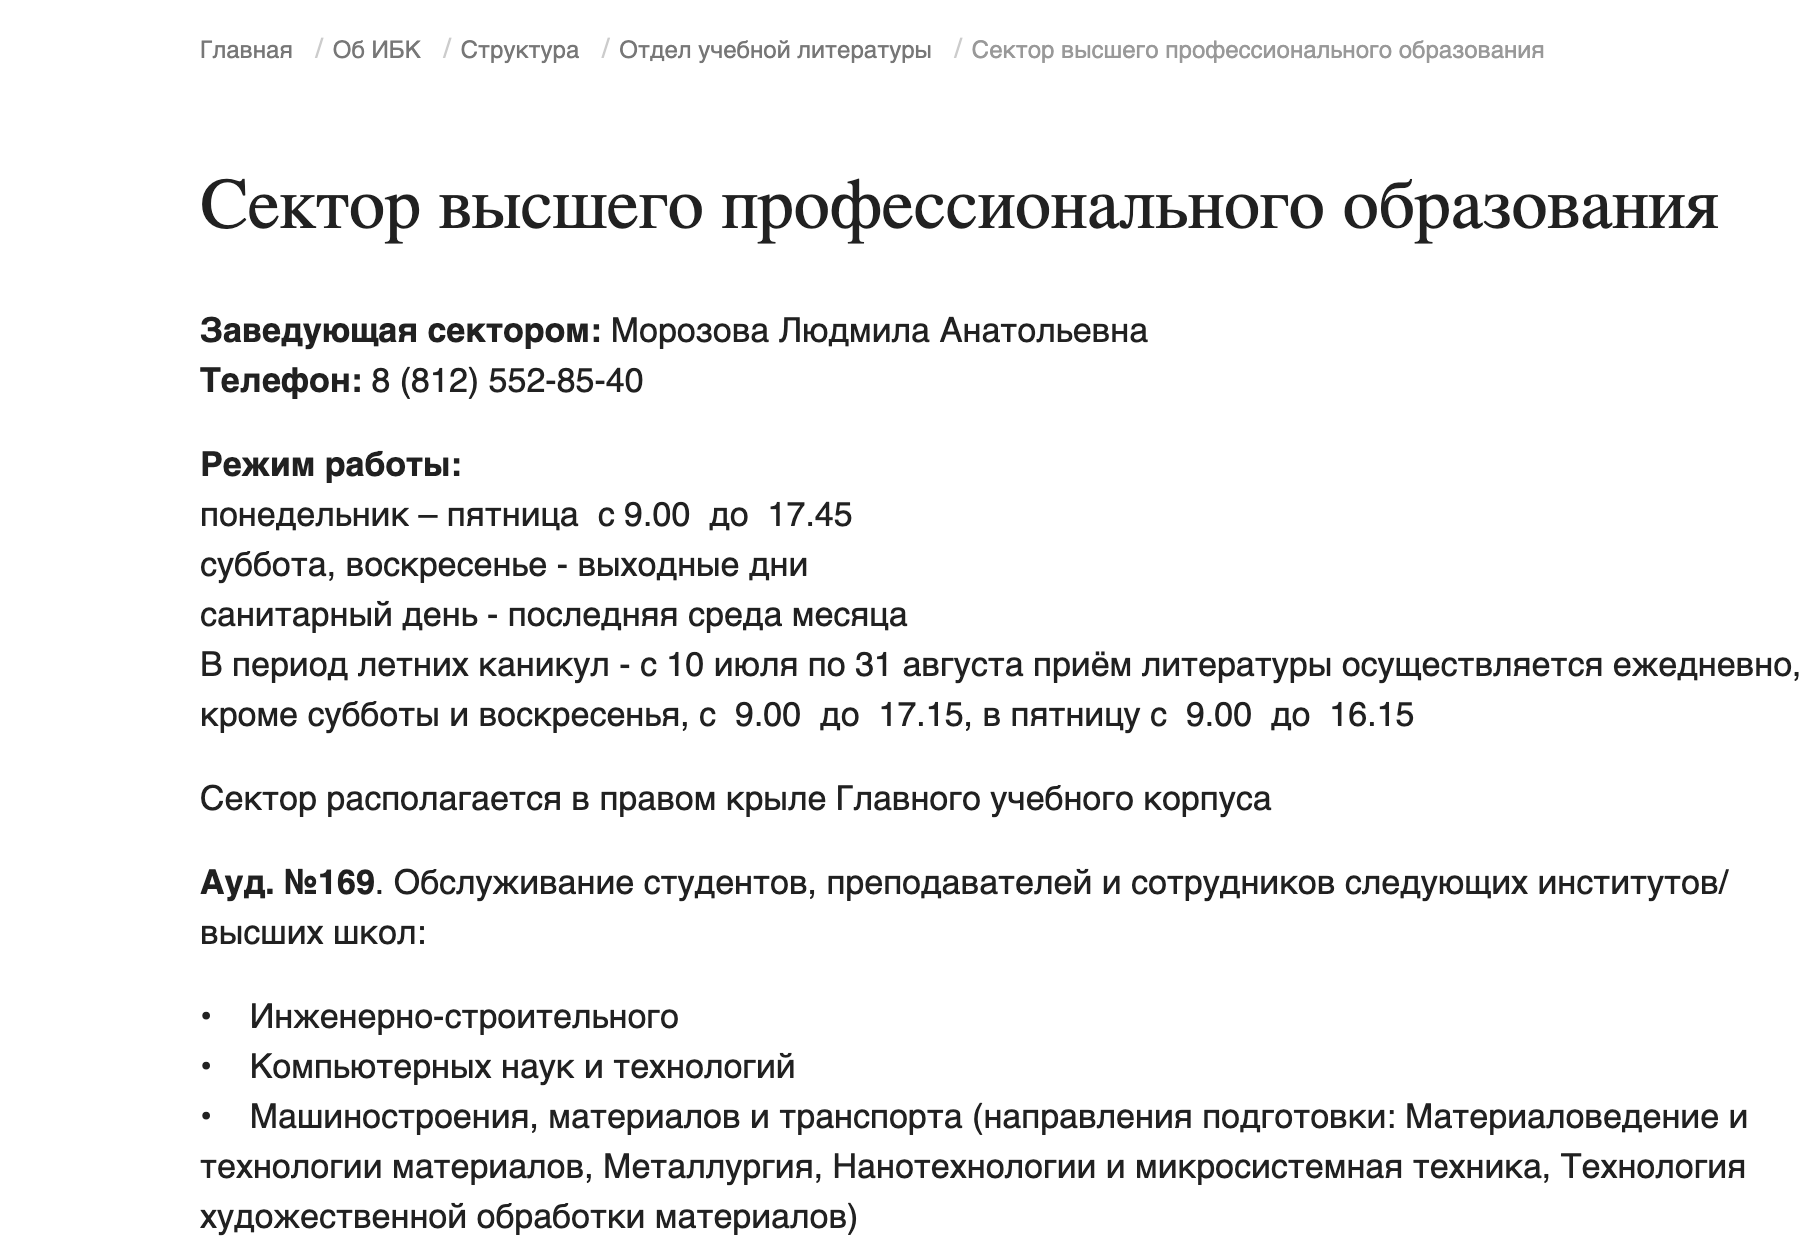
\includegraphics[scale = 0.5]{122.png}
\caption{Фрагмент структуры сектора ВПО отдела учебной литературы.}
\label{image:1}
\end{figure}

Далее на странице «Как нас найти», доступной через ссылку на главной странице или через пункт меню «Читателям» уточнили часы работы подразделения, перейдя по ссылке на данной странице на секторы, размещенные в Главном учебном корпусе.

\begin{figure}[h!]
\centering

\includegraphics[scale = 0.5]{123.png}
\caption{Поиск расположения подразделений библиотеки.}
\label{image:1}
\end{figure}

Самостоятельно определили расположение и расписание работы читальных залов библиотеки.

\begin{figure}[h!]
\centering

\includegraphics[scale = 0.5]{124.png}
\caption{Поиск расположения читальных залов.}
\label{image:1}
\end{figure}

\subsection{Упражнение 3. Поиск информационных ресурсов на библиотечном портале}

\subsubsection{Найти учебник, рекомендованный преподавателем, чтобы получить его для работы дома в течение семестра}

Поиск необходимого учебника выполняется в несколько шагов:

\begin{enumerate}
\item Выполняем анализ: какие страницы портала использовать для поиска требуемого ресурса. Поскольку все учебники, выдаваемые на дом, находятся в фонде библиотеки, то следует выполнять поиск на странице Электронного каталога.

\item Выполняем поиск учебника в электронном каталоге, например, учебника «Управление инновационными проектами», авторы которого - И. Л. Туккель, А. В. Сурина, Н. Б. Культин, опубликованного в 2014 г. в издательстве «БХВ-Петербург».

Ввели в строку поиска один из терминов по теме, фамилию хотя бы одного автора. Ввели запрос. Результаты поиска, после нескольких уточнений, будут выглядеть следующим образом.

\begin{figure}[h!]
\centering
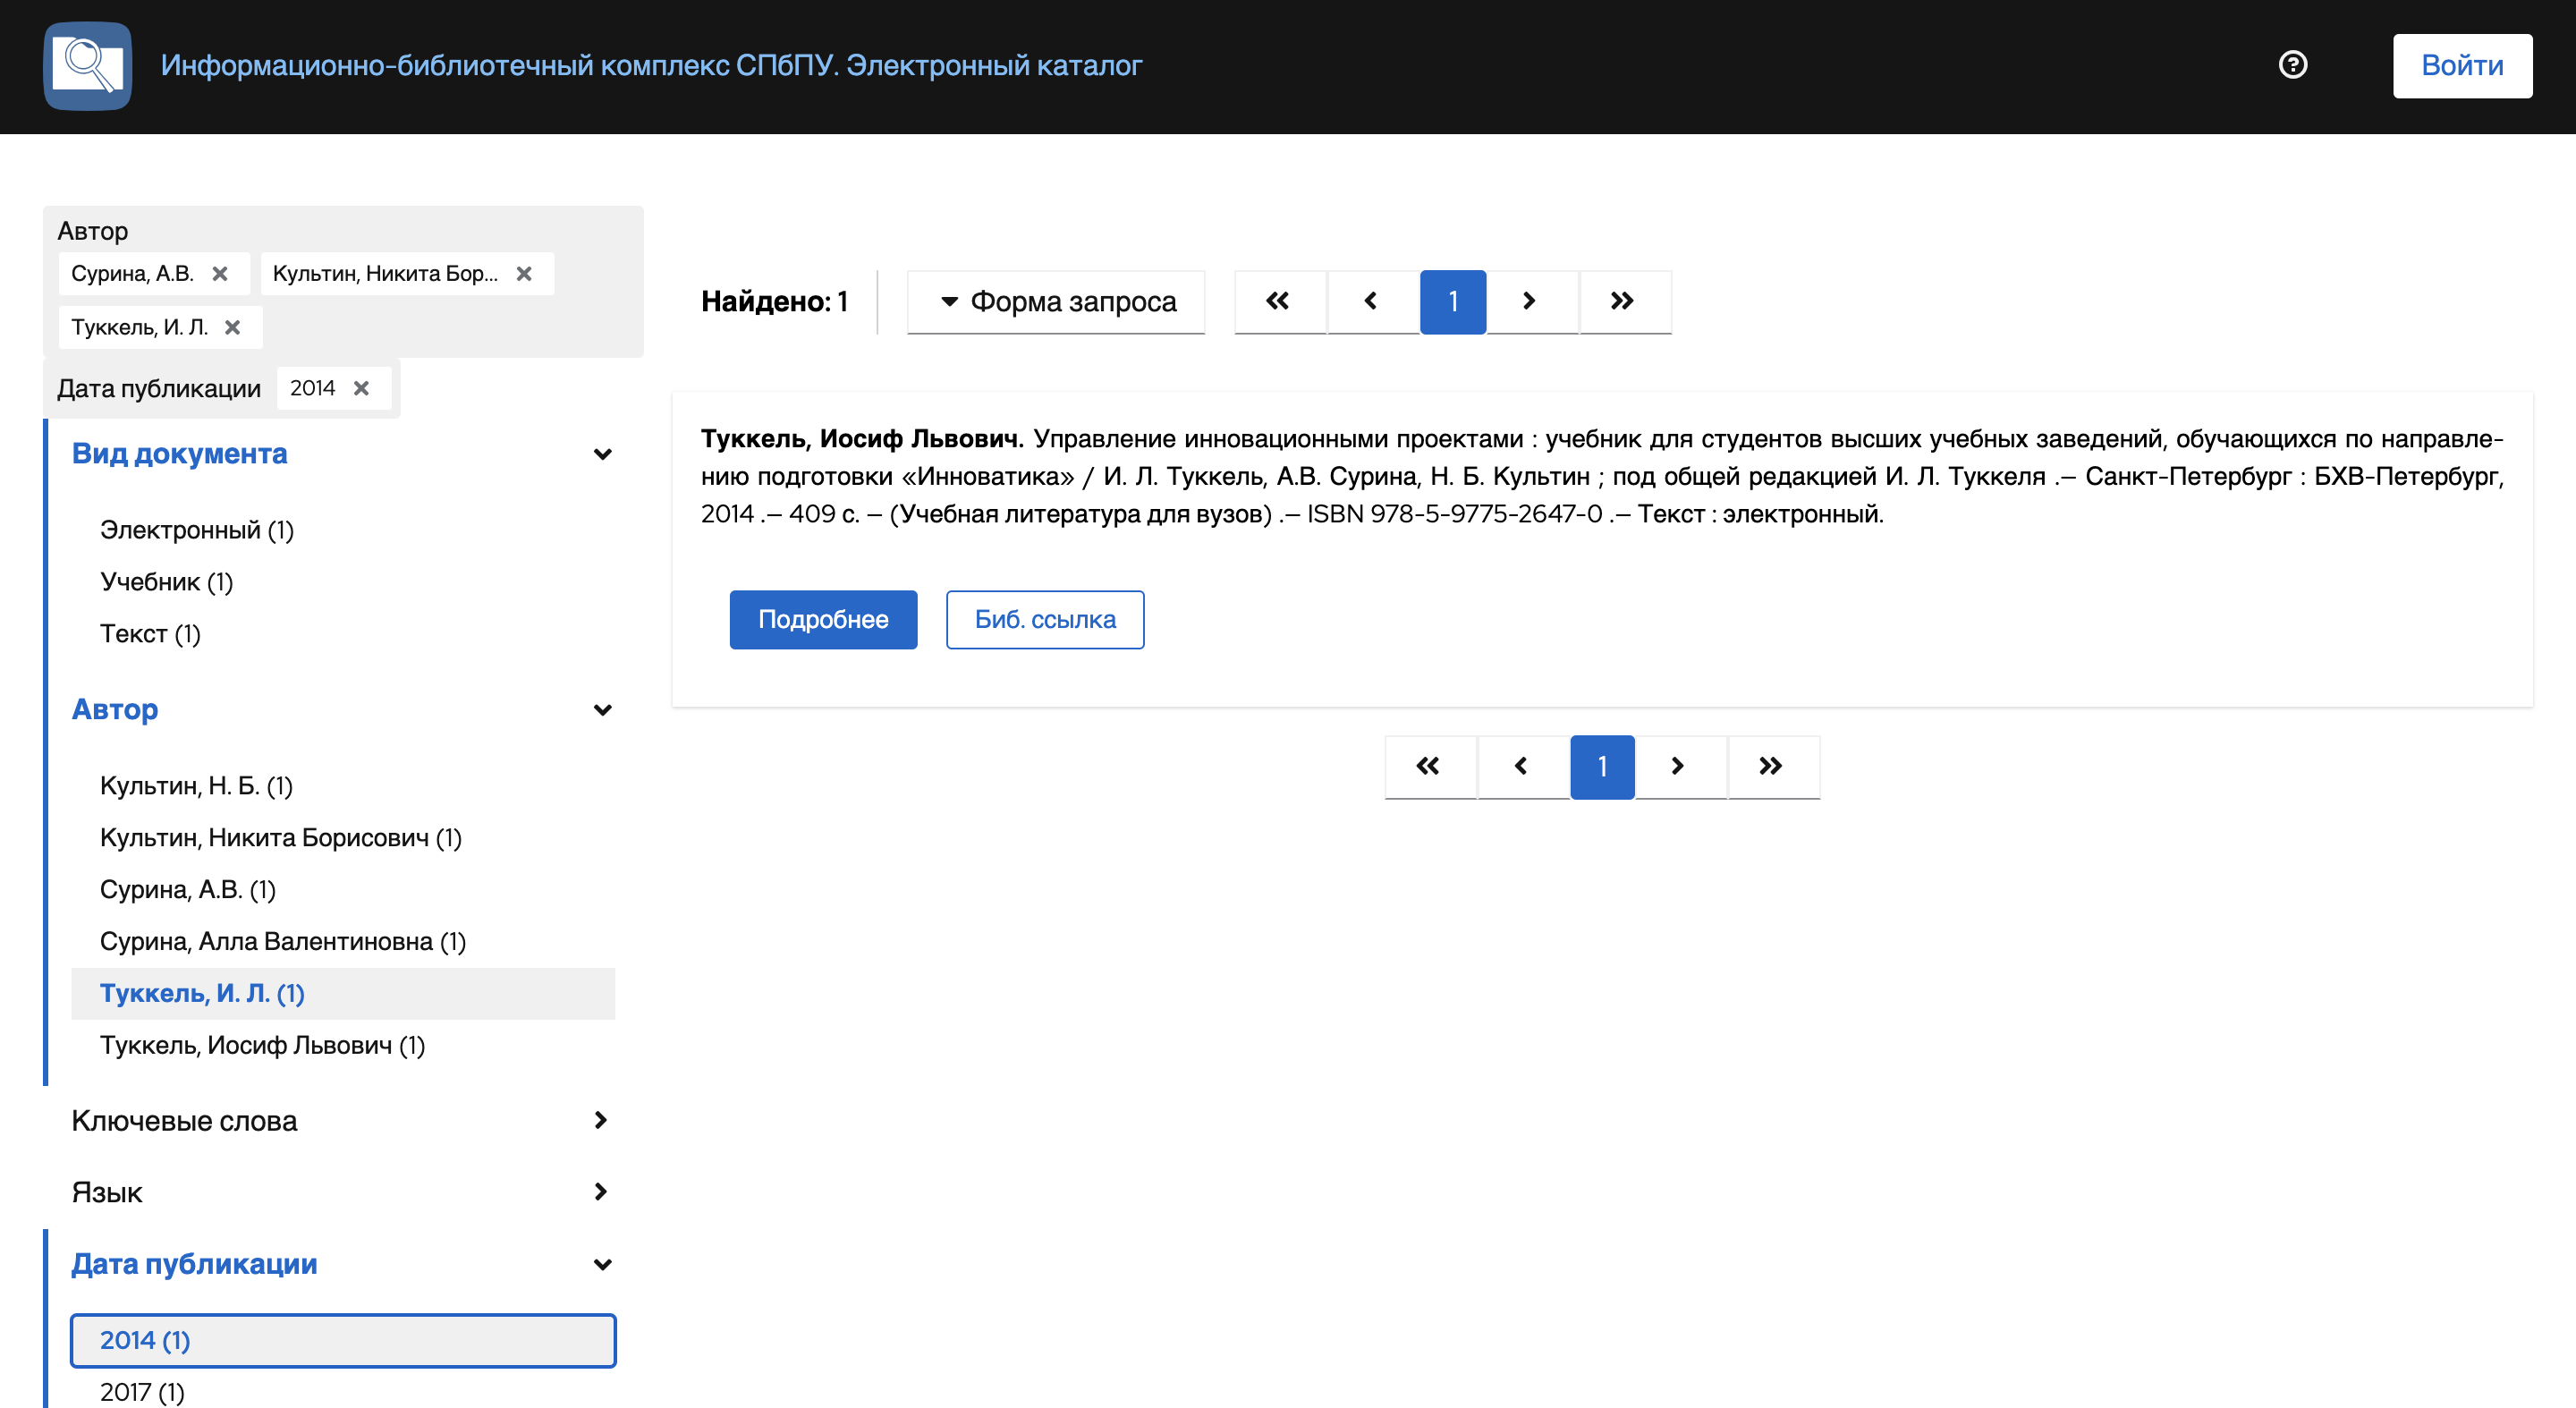
\includegraphics[scale = 0.33]{131.png}
\caption{Запрос на поиск учебника по инноватике.}
\label{image:1}
\end{figure}

Сначала в строку запроса было введено название учебника, причем можно вводить строчными буквами. Затем по фильтру (фасету) «Вид документа» был выбран «Учебник», были выбраны три нужных автора и год. После чего в списке найденных документов осталось всего 1 наименование

Выбирали рекомендованный - нажали на заглавие и перешли к детальному описанию учебника.

\item Изучили доступность учебника для получения. Видим, что в Отделе учебной литературы есть достаточное количество свободных экземпляров.

\item  Если требуется, по сайту уточняем расположение и часы работы отдела (см. выше)
\end{enumerate}

\clearpage

Самостоятельно нашли, где можно получить учебник по термодинамике. Выбрали издания, опубликованные за последние 5 лет.

\begin{figure}[h!]
\centering
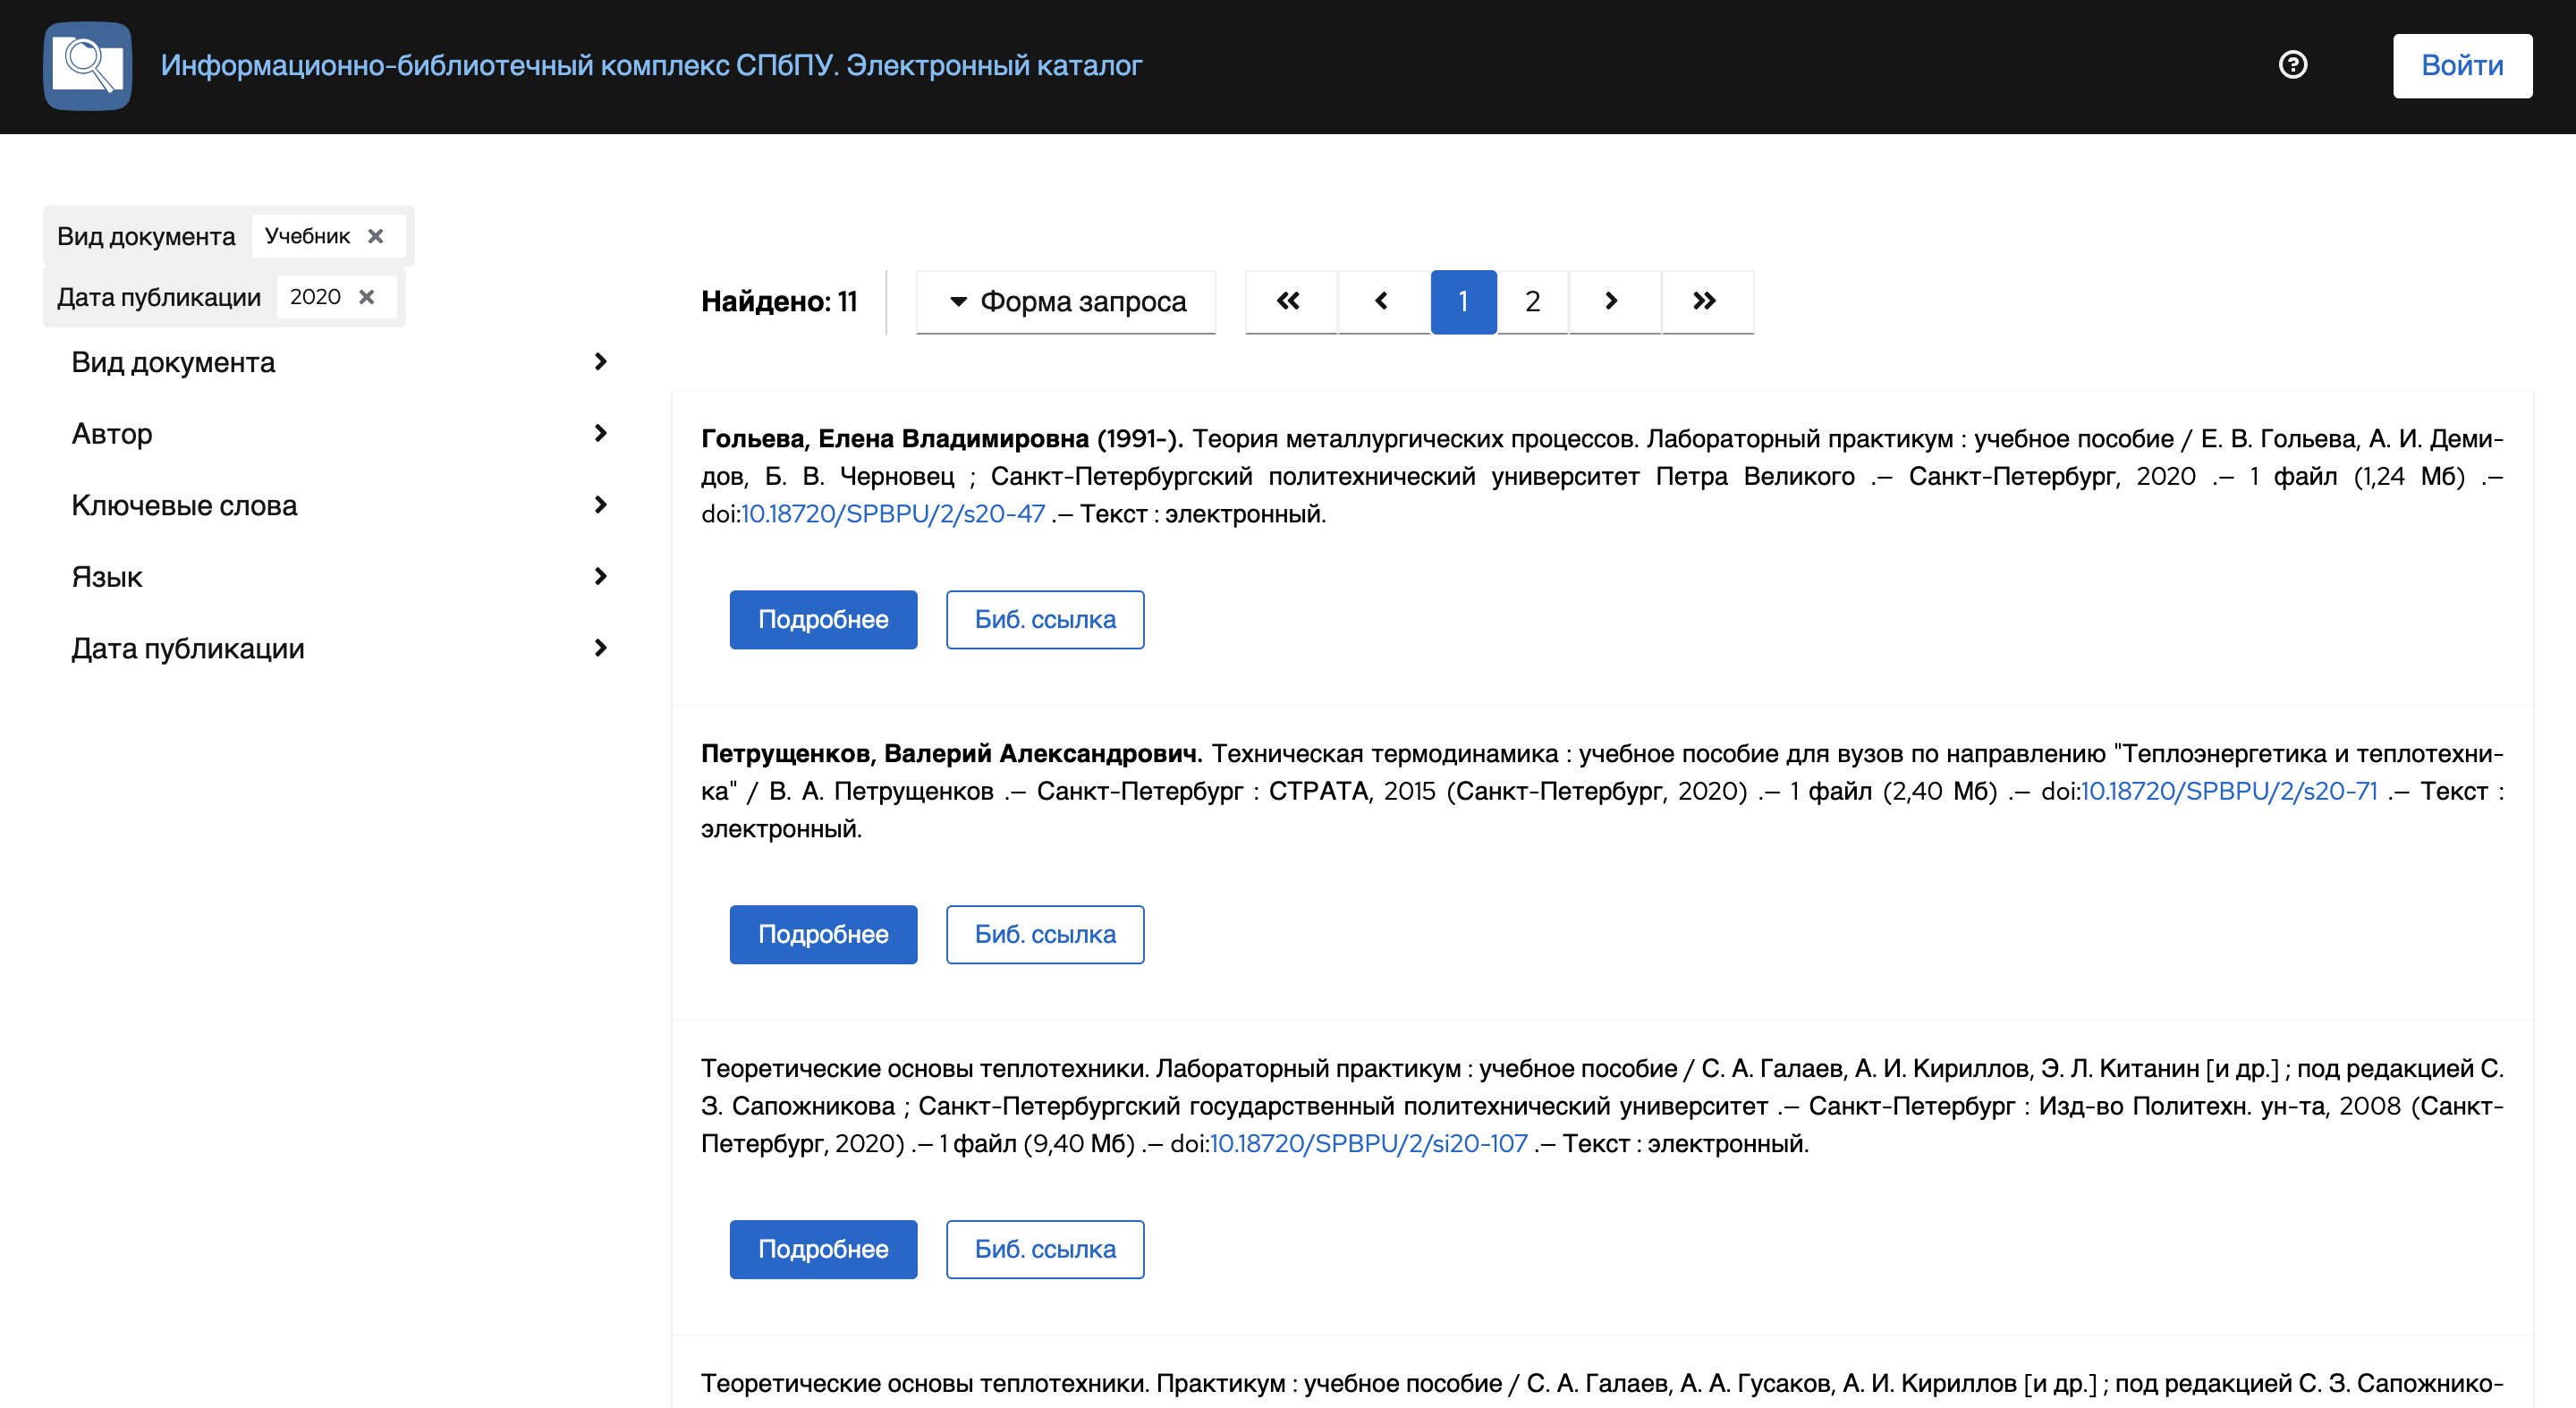
\includegraphics[scale = 0.33]{132.png}
\caption{Запрос на поиск учебника по темодинамике.}
\label{image:1}
\end{figure}

Запрос был выполнен с текстом "Термодинамика". После чего были применены фильтры "Вид документа" - "Учебник", а также "Дата публикации" - "2020".

Возможность просмотра состояния наличия учебников отсутствует в связи с тем, что нет доступа к ИКБ.

\subsubsection{Найти учебно-методическую литературу в базах данных по экономике, доступную в электронном виде через Интернет.}

\begin{enumerate}
\item Выполнили анализ: какие страницы портала использовать для поиска требуемого ресурса. Учебные издания следует искать на страницах Электронного каталога или Электронной библиотеки. Поскольку требуются учебные издания, доступные в Интернет, то целесообразно воспользоваться интерфейсом ЭБ, где доступность в Интернет отражена в одном из фасетов.
\item Выполнили поиск. Для этого ввели в строке поиска следующие термины

\begin{figure}[h!]
\centering

\includegraphics[scale = 0.33]{133.png}
\caption{Запрос на поиск литературы в ЭБ СПбПУ и ЭБС.}
\label{image:1}
\end{figure}

Оценили результаты. Найдено 22 868 ресурсов – это слишком много для последовательной оценки найденных ресурсов. Уточнили запрос – выбрали коллекцию «Учебная и учебно- методическая литература в фасете «Коллекция». Теперь найдено 1 355 ресурса. Уточнили запрос – выбрали только доступные из Интернет по паролю читателя, используя фасет «Доступ». Теперь найдено 232 ресурсов. Можно продолжать фильтрацию, а можно оценить первые в списке ресурсы – ведь при выводе результатов происходит их сортировка по релевантности. На первой странице нашли текст лекций по курсу "Информационные системы в экономике". Проверили, соответствует ли этот ресурс по своему содержанию нашим требованиям.

\clearpage

\item Перешли к детальному описанию. Изучили аннотацию, содержание.
\item Уточнили сведения о доступности – он доступен из Интернет по паролю читателя.

\begin{figure}[h!]
\centering
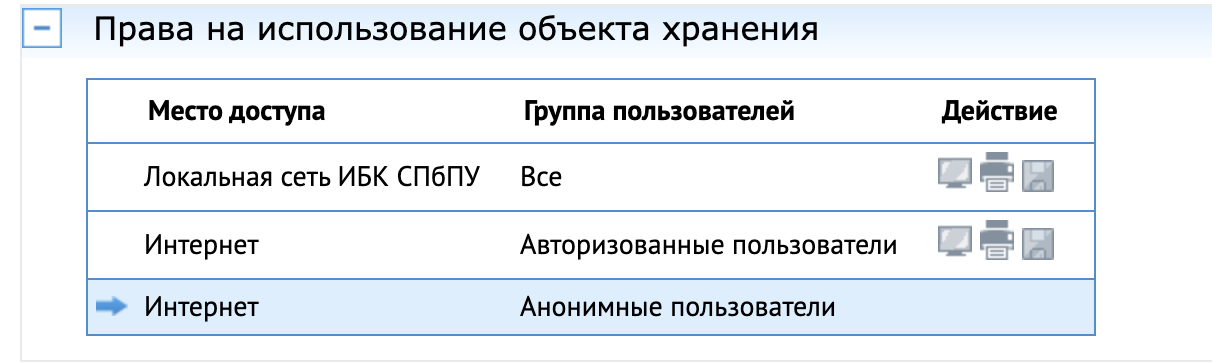
\includegraphics[scale = 0.33]{134.png}
\caption{Права на использование учебного издания в ЭБ СПбПУ.}
\label{image:1}
\end{figure}

\end{enumerate}

Все условия, предъявляемые при поиске ресурса, выполнены. Задача решена.

Самостоятельно нашли пособия по решению задач по термодинамике. Выбрали доступные в Интернет по паролю читателя. Выбрали рекомендованные для нашего направления подготовки.


\begin{figure}[h!]
\centering

\includegraphics[scale = 0.33]{135.png}
\caption{Результат запроса поиска литературы в ЭБ СПбПУ и ЭБС.}
\label{image:1}
\end{figure}

\begin{figure}[h!]
\centering
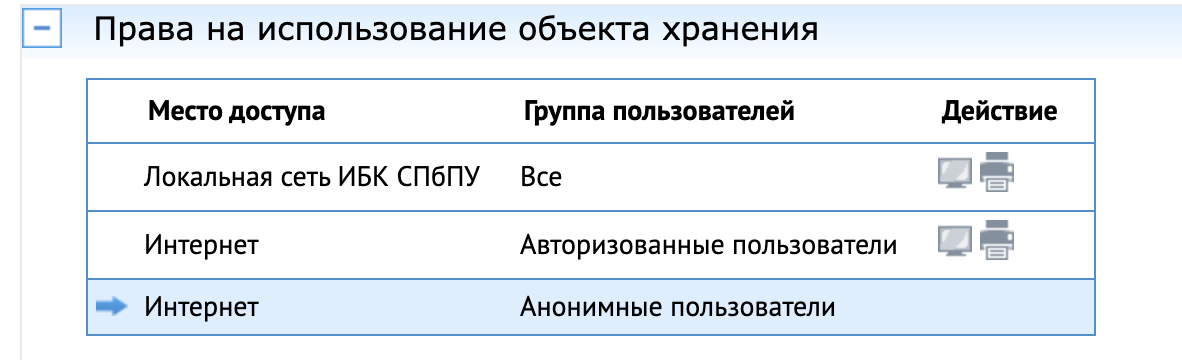
\includegraphics[scale = 0.33]{136.png}
\caption{Права на использование учебного издания в ЭБ СПбПУ.}
\label{image:1}
\end{figure}

\subsubsection{Найти актуальную литературу по блокчейну для написания обзора.}

\begin{enumerate}
\item Выполнили анализ: какие страницы портала использовать для поиска требуемого ресурса. Поскольку для обзора важна актуальная информация, то требуются разнообразные ресурсы, в том числе статьи из научных журналов, значит, нам потребуются все доступные источники: электронный каталог, ресурсы российских и зарубежных баз данных.
\item Поиск по электронному каталогу – ввели «блокчейн» в окно поиска. Найдено 38 документов, в том числе 21 выпускных квалификационных работ в ЭБ, доступные из Интернет.
Продолжили поиск в ЭБ – там поиск расширен за счет поиска искомых терминов в тексте документа. Найдено 378, из них доступны в интернет лишь 111.
Продолжили поиск в российских БД – "На сервере возникла ошибка. Отчет об ошибке направлен администраторам.".
Продолжили поиск в зарубежных БД - "The page you have tried to access has expired, please return to your Library home page to restart a session on EBSCOhost".
\end{enumerate}

\clearpage

\subsubsection{Найти один из нормативных документов в выбранной области, например, по дорожному строительству.}

\begin{enumerate}
\item Выполнили анализ: нормативные ресурсы размещаются в специализированных базах данных. Значит, следует проводит поиск базы данных на странице «Базы данных».
\item По фасету «Вид документа» выбираем «нормативно-технические».

\begin{figure}[h!]
\centering
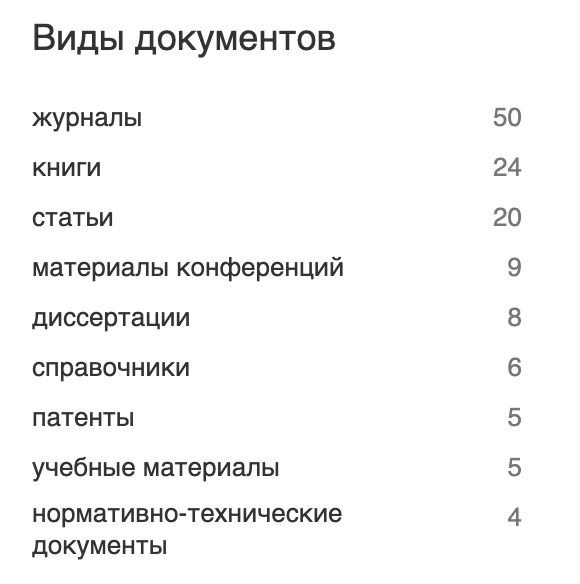
\includegraphics[scale = 0.33]{137.png}
\caption{Раскрытие содержимого БД по виду документов.}
\label{image:1}
\end{figure}

Сделали предварительную оценку возможности нахождения в них требуемых документов.

\begin{figure}[h!]
\centering
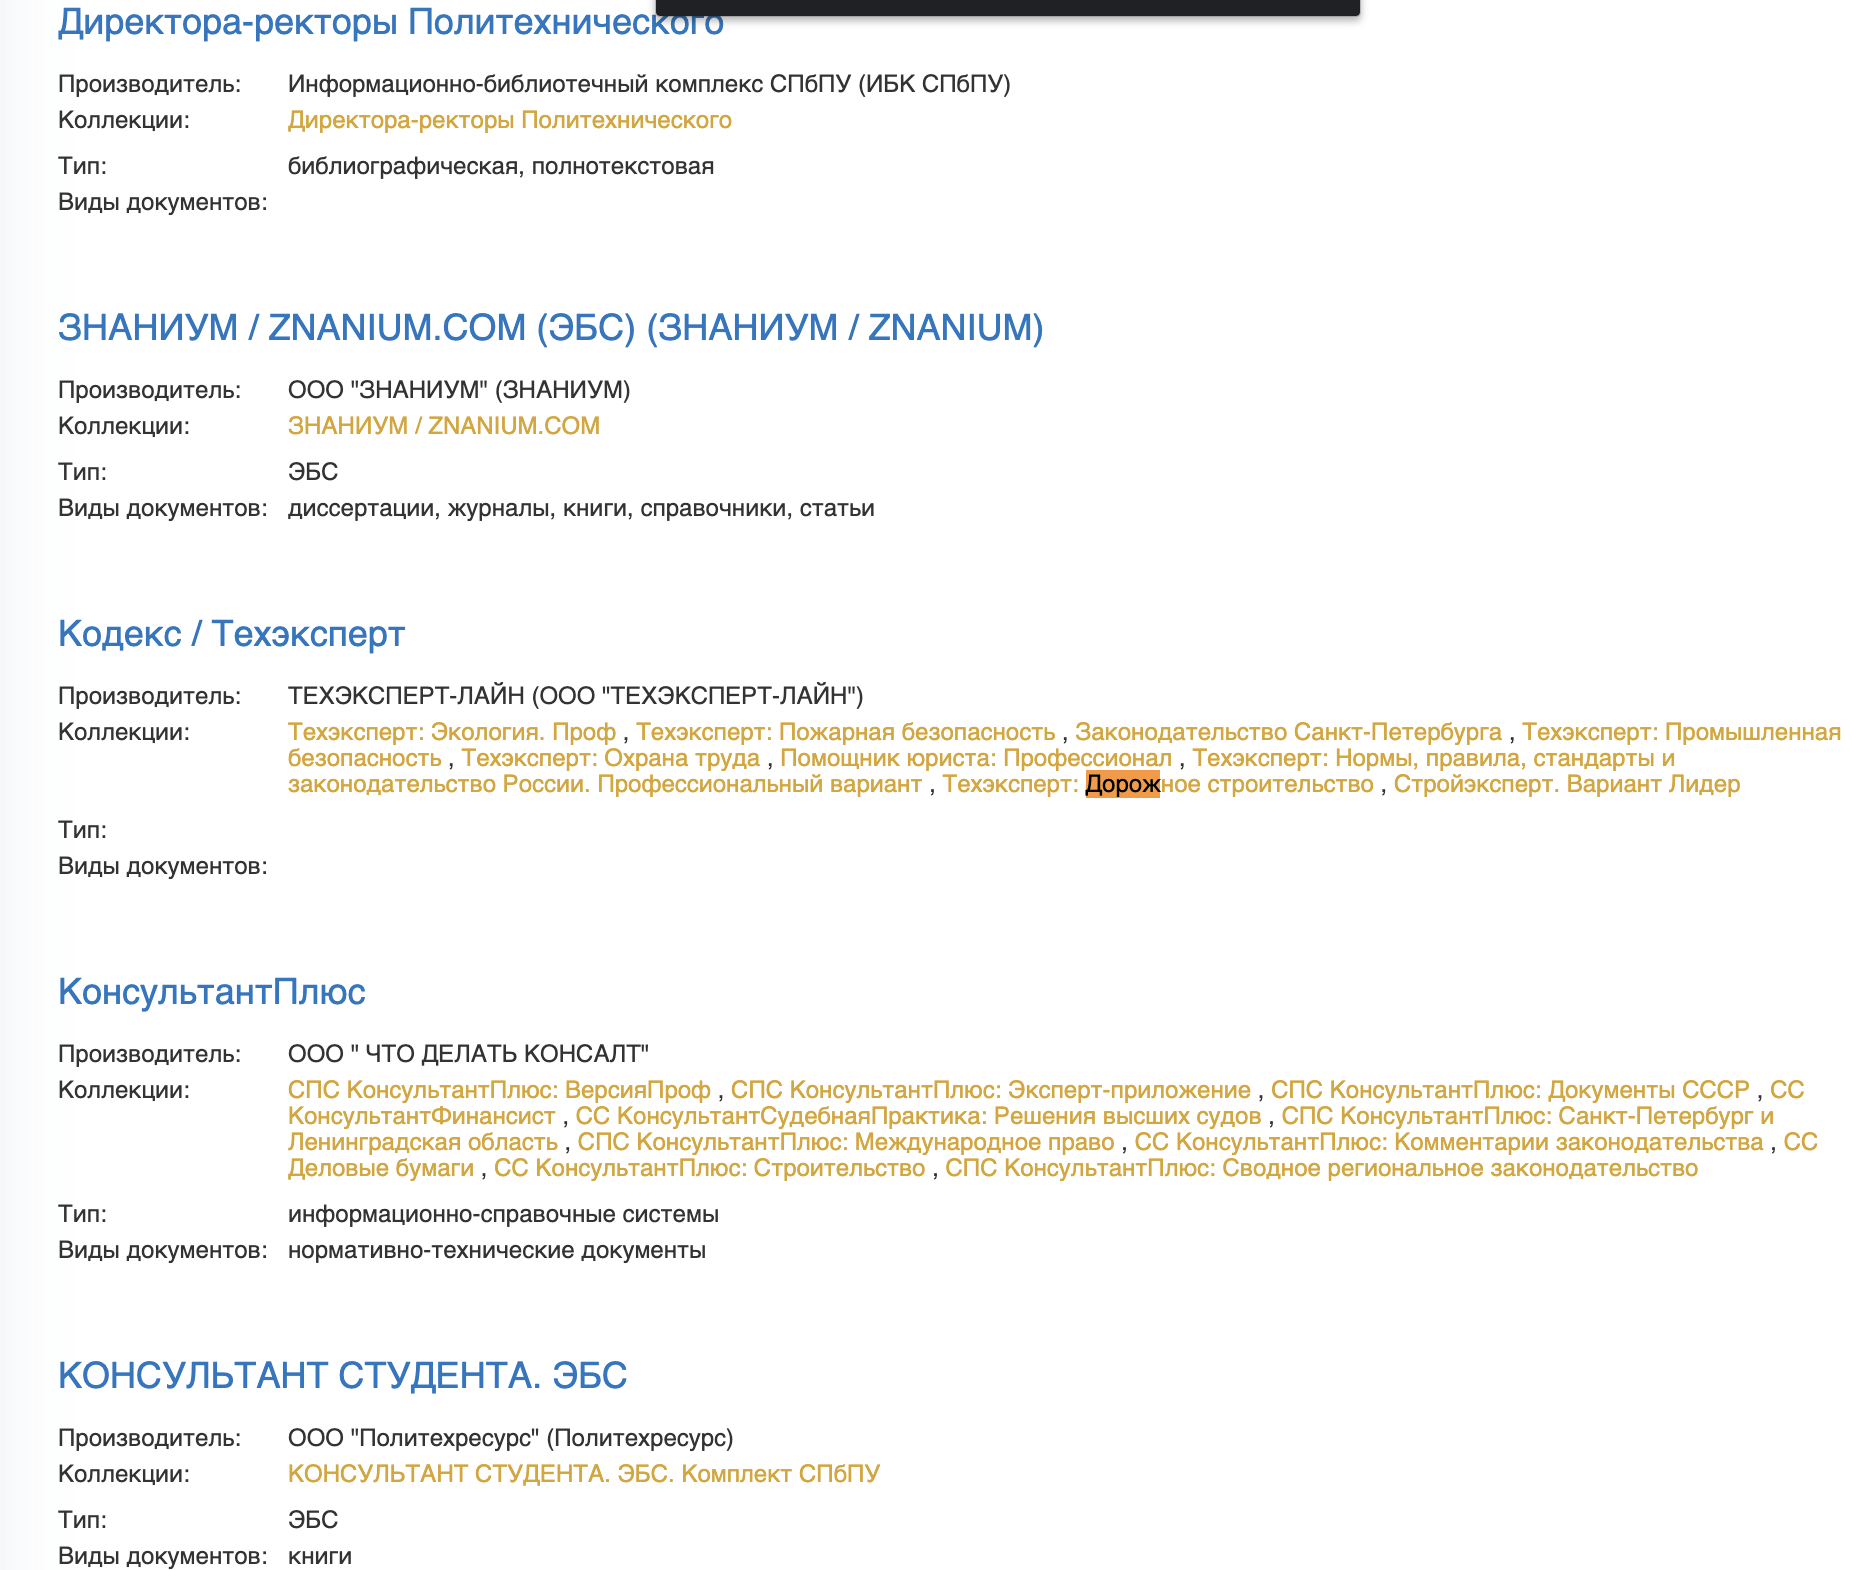
\includegraphics[scale = 0.33]{138.png}
\caption{Фрагмент результатов поиска баз данных.}
\label{image:1}
\end{figure}

\item Перешли к детальному описанию базы. Уточнили, каким образом база доступна для использования.
\item Выполнили поиск требуемого постановления в интерфейсе (на платформе) выбранной базы данных.
\end{enumerate}

Самостоятельно нашли информацию по патентам в области химии.

\begin{figure}[h!]
\centering
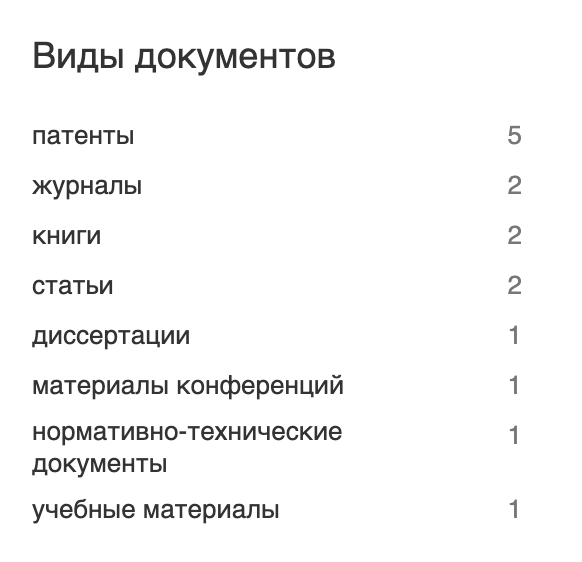
\includegraphics[scale = 0.33]{139.png}
\caption{Фрагмент результатов поиска баз данных.}
\label{image:1}
\end{figure}

\begin{figure}[h!]
\centering
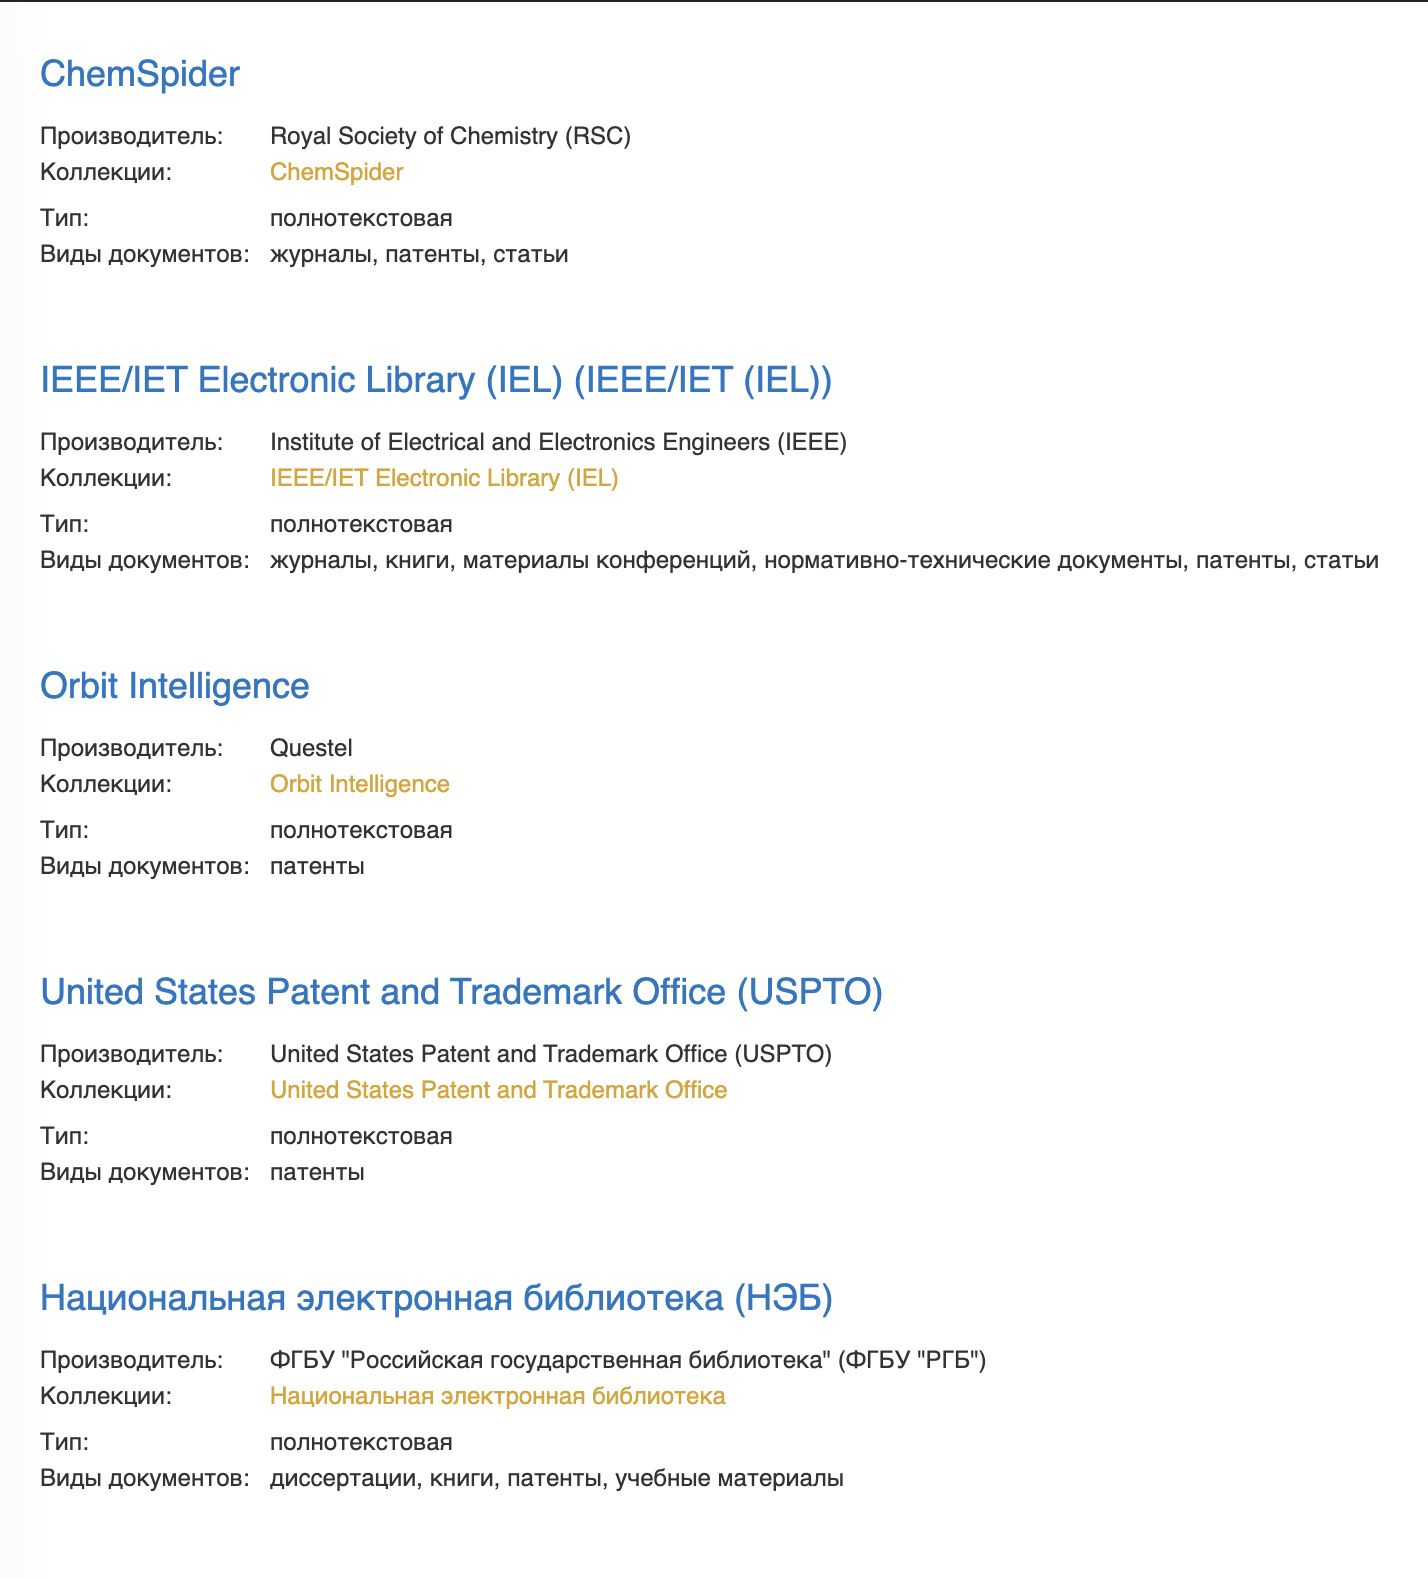
\includegraphics[scale = 0.33]{1310.png}
\caption{Фрагмент результатов поиска баз данных.}
\label{image:1}
\end{figure}

\begin{figure}[h!]
\centering
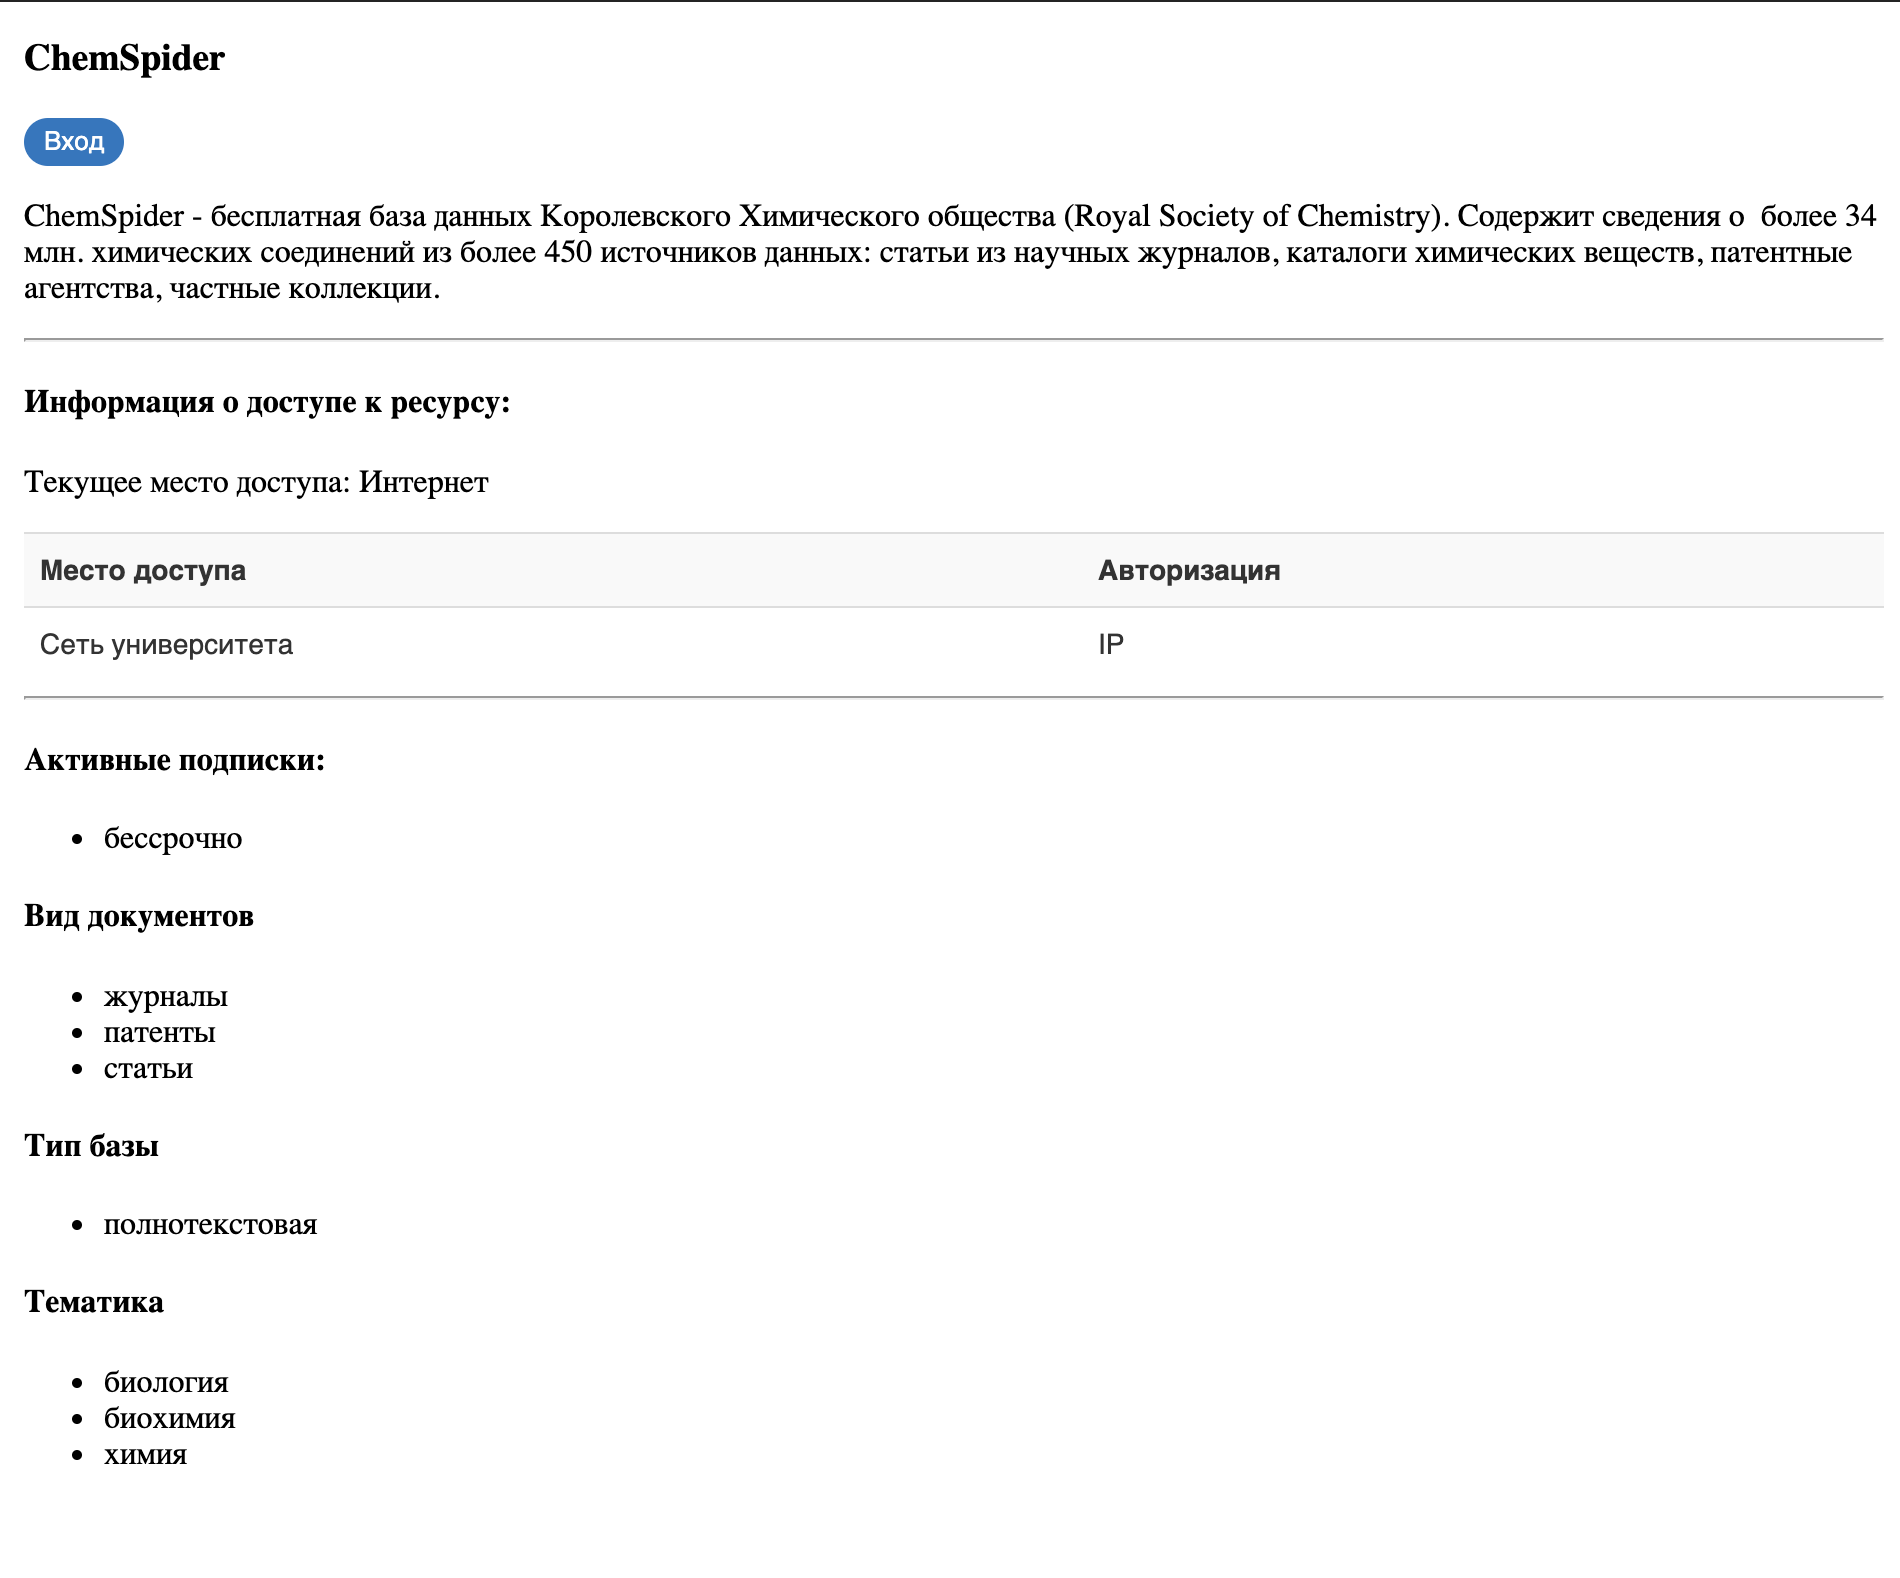
\includegraphics[scale = 0.33]{1311.png}
\caption{Фрагмент результатов поиска баз данных.}
\label{image:1}
\end{figure}

\section{Вывод}
В ходе проделанной практической работы были получены навыки работы с библиотечным сайтом.
\clearpage

\end{document}